\section{Der FreeDesign-Editor}
\label{Der FreeDesign-Editor}
\subsection{Funktionsbeschreibung}
Der, durch Unitedprint bereitgestellte, Webshop \emph{easyprint.com} bietet Kunden die Möglichkeit Druckprodukt online zu gestaltet und im Anschluss zu bestellen. Für die Gestaltung der Produkte wurde unternehmenintern die Webanwendung \emph{FreeDesign} entwickelt, welche beständig gepflegt und weiterentwickelt wird. Die Anwendung ist eine Single-Page-Webanwendung, welche in der Programmiersprache TypeScript, sowie unter der Verwendung von \emph{ReactJS} und \emph{Redux} entwickelt wurde. 

Basierend auf Flanagan (\citeyear[S. 497]{Flanagan2006}) wird als Single-Page-Webanwendung ein Webanwendung bezeichnet die auf der Ajax-Technologie basiert und ihre Inhalt per JavaScript aktualisiert und nicht durch das neu Laden der Anwendung. 

Mit hilfe des Editor kann eine große Vielzahl von Druckprodukten gestaltet werden, wobei das Portfolio verschiedenste Produktgruppen, wie Bürozubehör, Textilien oder Werbematerialien, abdeckt. Zur Gestaltung eines Designs bietet der Editor die Möglichkeit der Nutzung eigener Text und Bilder sowie das Verwenden verschiedenster geometrischer Formen. Alle Element können umfangreich geometrisch und grafische bearbeitet werden. Um einen optimalen Gestaltungsprozess zu ermöglichen, kann die Produktdarstell auch wärend der Gestaltung vergrößert, verschoben oder rotiert werden. Weiterhin stehen auch Hilfwerkzeuge wie Lineal oder Hilflinien zur Verfügung. 

Die Nutzer haben auch die Möglichkeit Designs als Entwürfe zu speicheren und zu einem späteren Zeitpunkt zu öffnen.

\begin{figure}[H]
    \centering
    \efbox{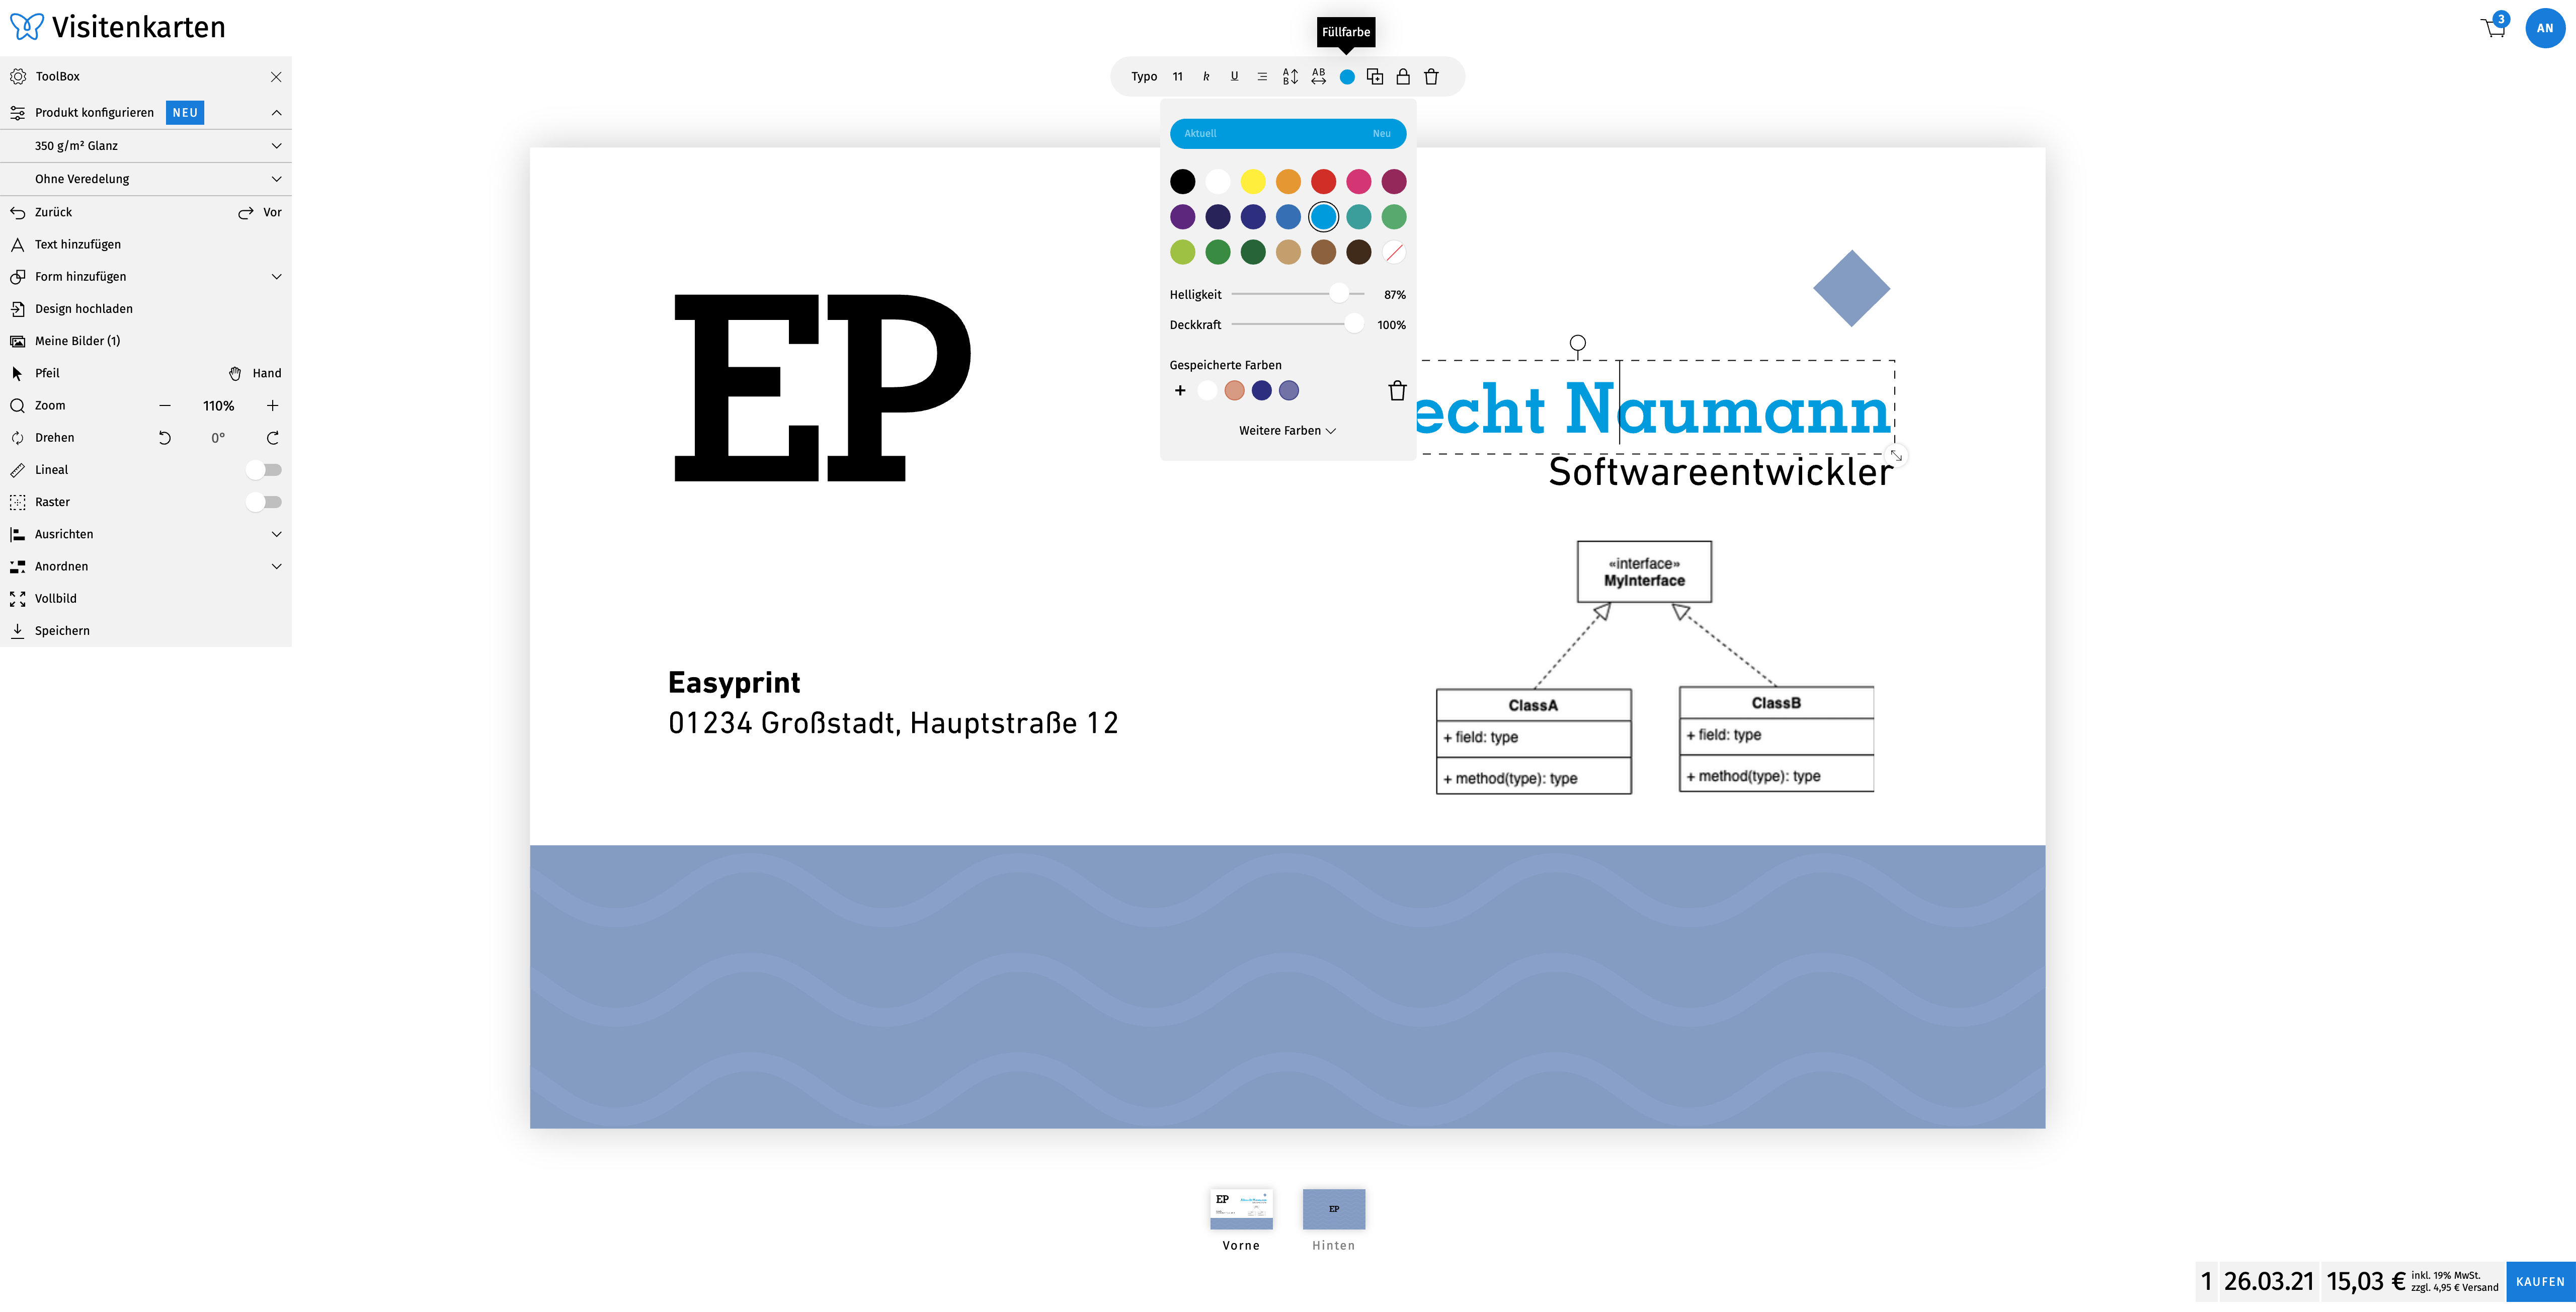
\includegraphics[width=.98\textwidth]{chapter/freedesign/Screenshot-Freedesign.png}}
    \caption{Ein Bildschirmfoto des FreeDesign-Editor}
    \label{fig:Der FreeDesign-Editor}
\end{figure}

\subsection{Designvorlagen}

\begin{figure}[H]
    \centering
    \efbox{\includegraphics[width=.98\textwidth]{chapter/freedesign/Screenshot-Designseite.png}}
    \caption{Ein Bildschirmfoto der Designübersichtseite für Visitenkarten}
    \label{fig:Designuebersichtseite}
\end{figure}

\begin{figure}[H]
    \centering
    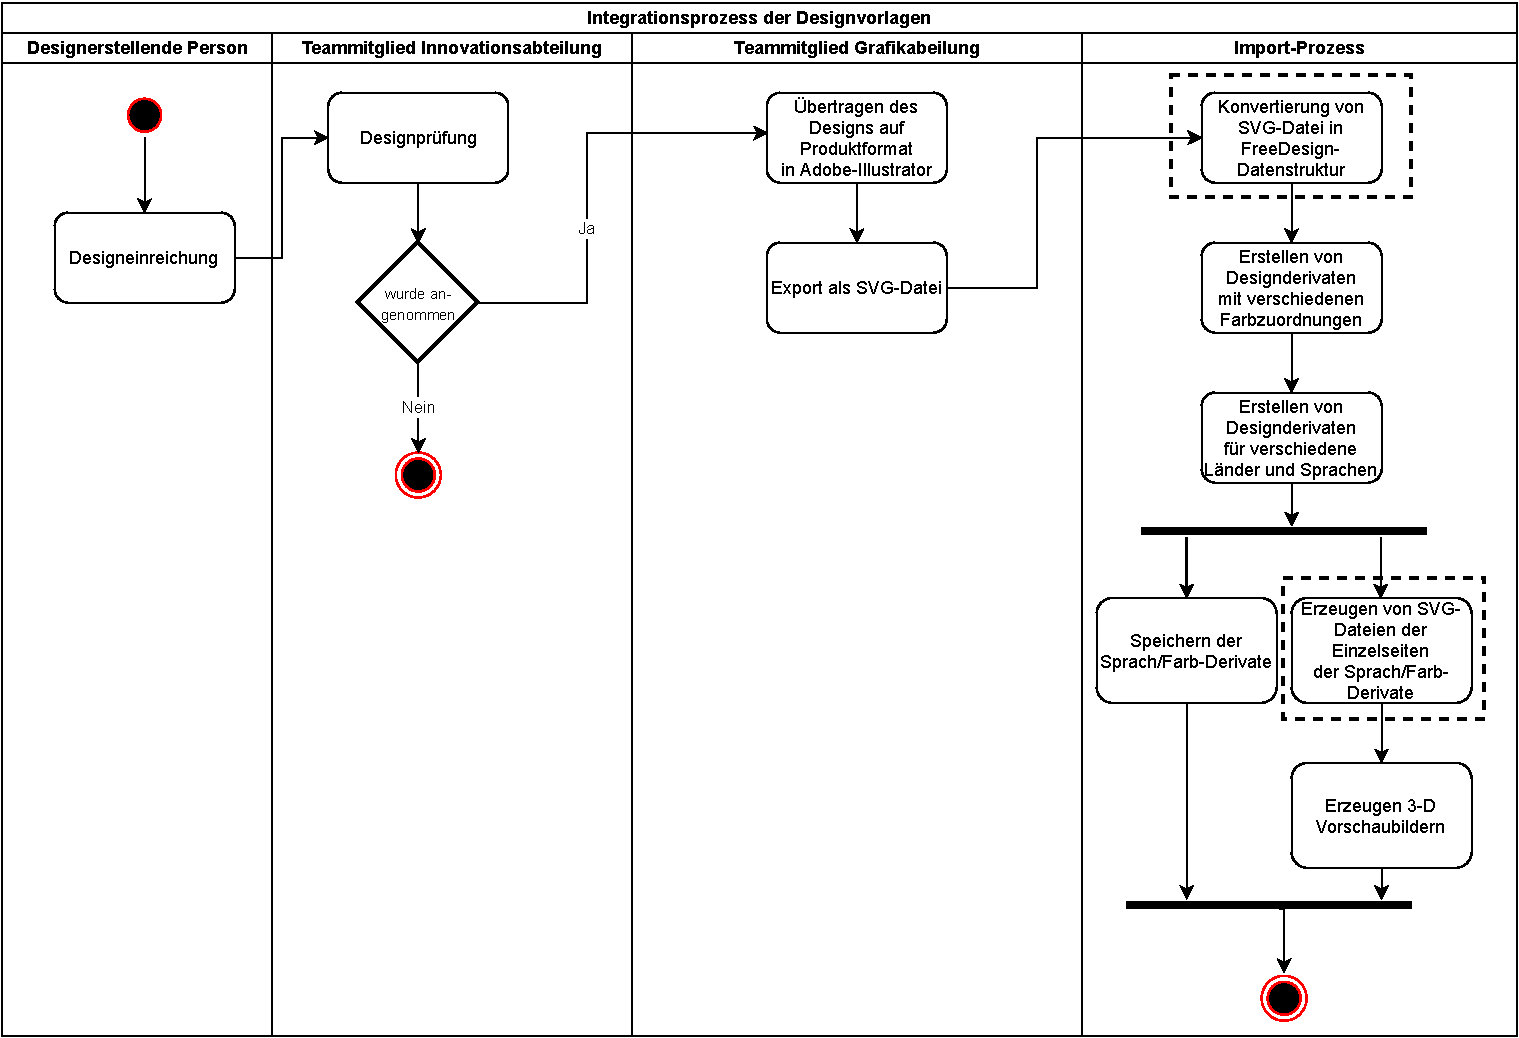
\includegraphics[width=.98\textwidth]{diagrams/Freedesign-Vorlagenerstellung.pdf}
\caption{Prozessbeschreibung der Vorlagenerstellung}
\label{fig:Vorlagenimport}
\end{figure}

\subsection{Bestellablauf}
%TODO: => Auf Team eingehen

